%**************************************************************************************************************
\subsection{\gls[hyper=false]{gp} \gls[hyper=false]{pc} Metamodel Construction}\label{sub:gp_feba_pc_metamodel}
%**************************************************************************************************************

\begin{sidewaysfigure}
	\centering
	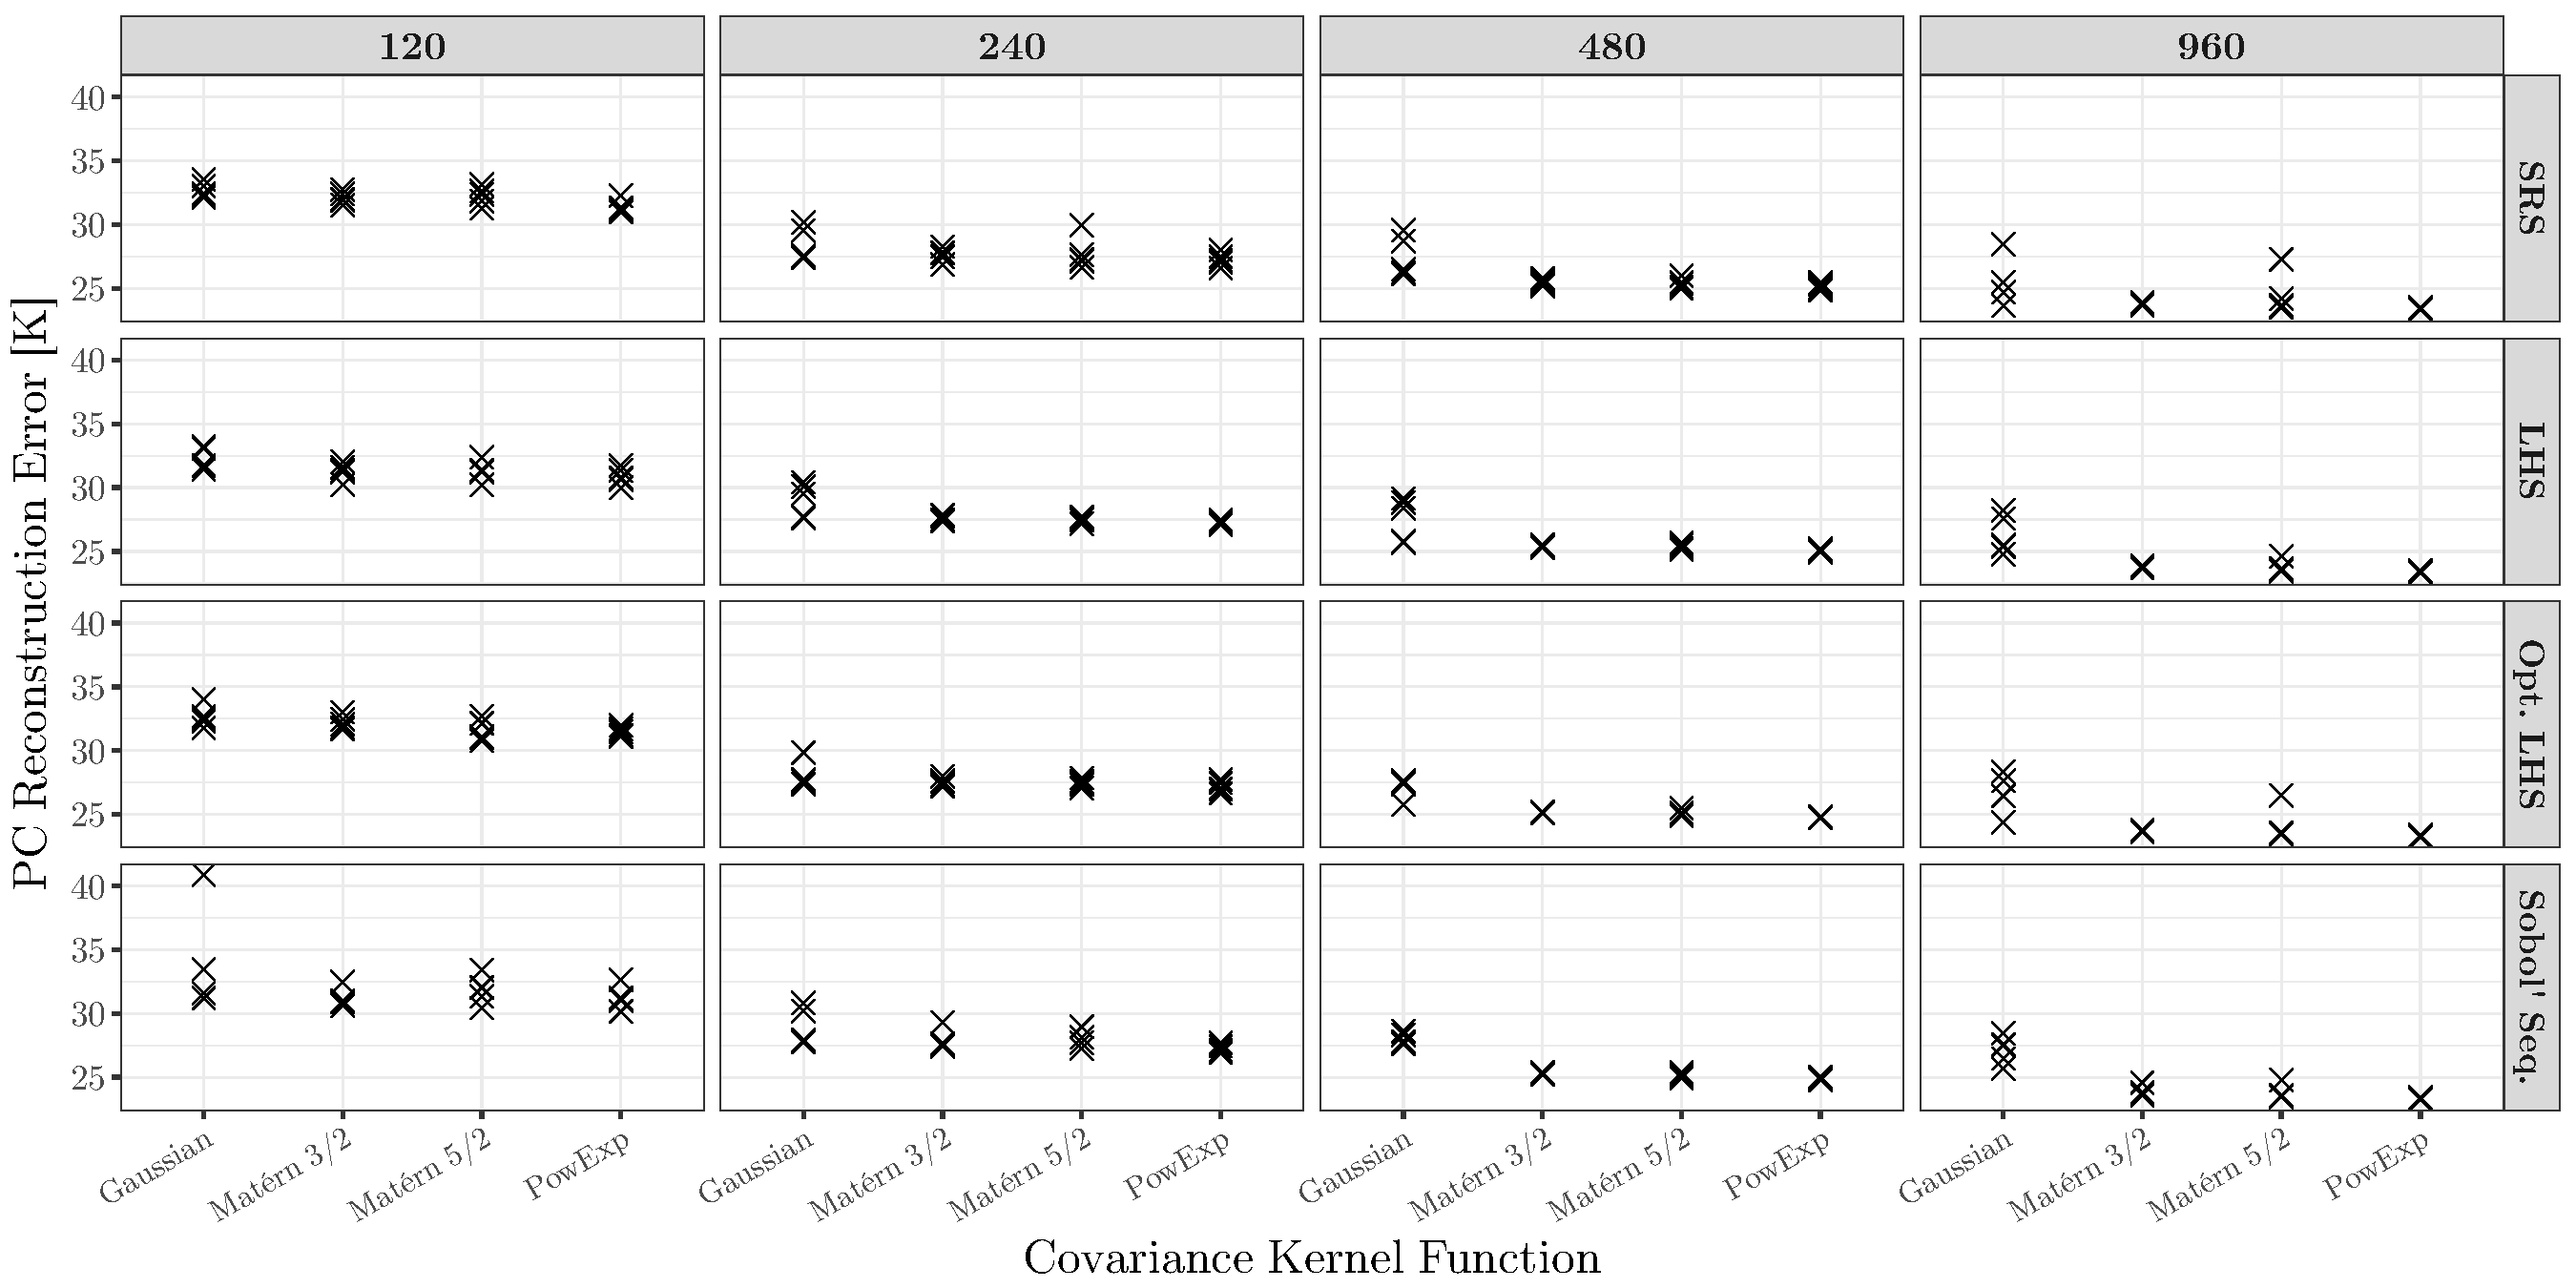
\includegraphics[width=1.0\textwidth]{../figures/chapter4/figures/plotPCGPConstructionTC}
	\caption[The flowchart for the implemented sensitivity analysis methodology applied to the TRACE model of FEBA facility]{The flowchart for the implemented sensitivity analysis methodology applied to the \gls{trace} model of \gls{feba} facility}
	\label{fig:ch4_plot_pc_gp_construction_tc}
\end{sidewaysfigure}

\bigfigure[pos=!tbhp,
					 opt={width=1.0\textwidth},
           label={fig:ch4_plot_pc_q2_tc},
           shortcaption={Sobol' Indices estimates with the scores of the warping function for the mid-height clad temperature transient as the \gls[hyper=false]{qoi}}]
{../figures/chapter4/figures/plotPCQ2TC}
{The sensitivity indices with respect to theof the warping function for the mid-height clad temperature transient. Each boxplot represents the bootstrap sample quartile statistics and the vertical line extends the $95$th sample percentile.}

\begin{sidewaysfigure}
	\centering
	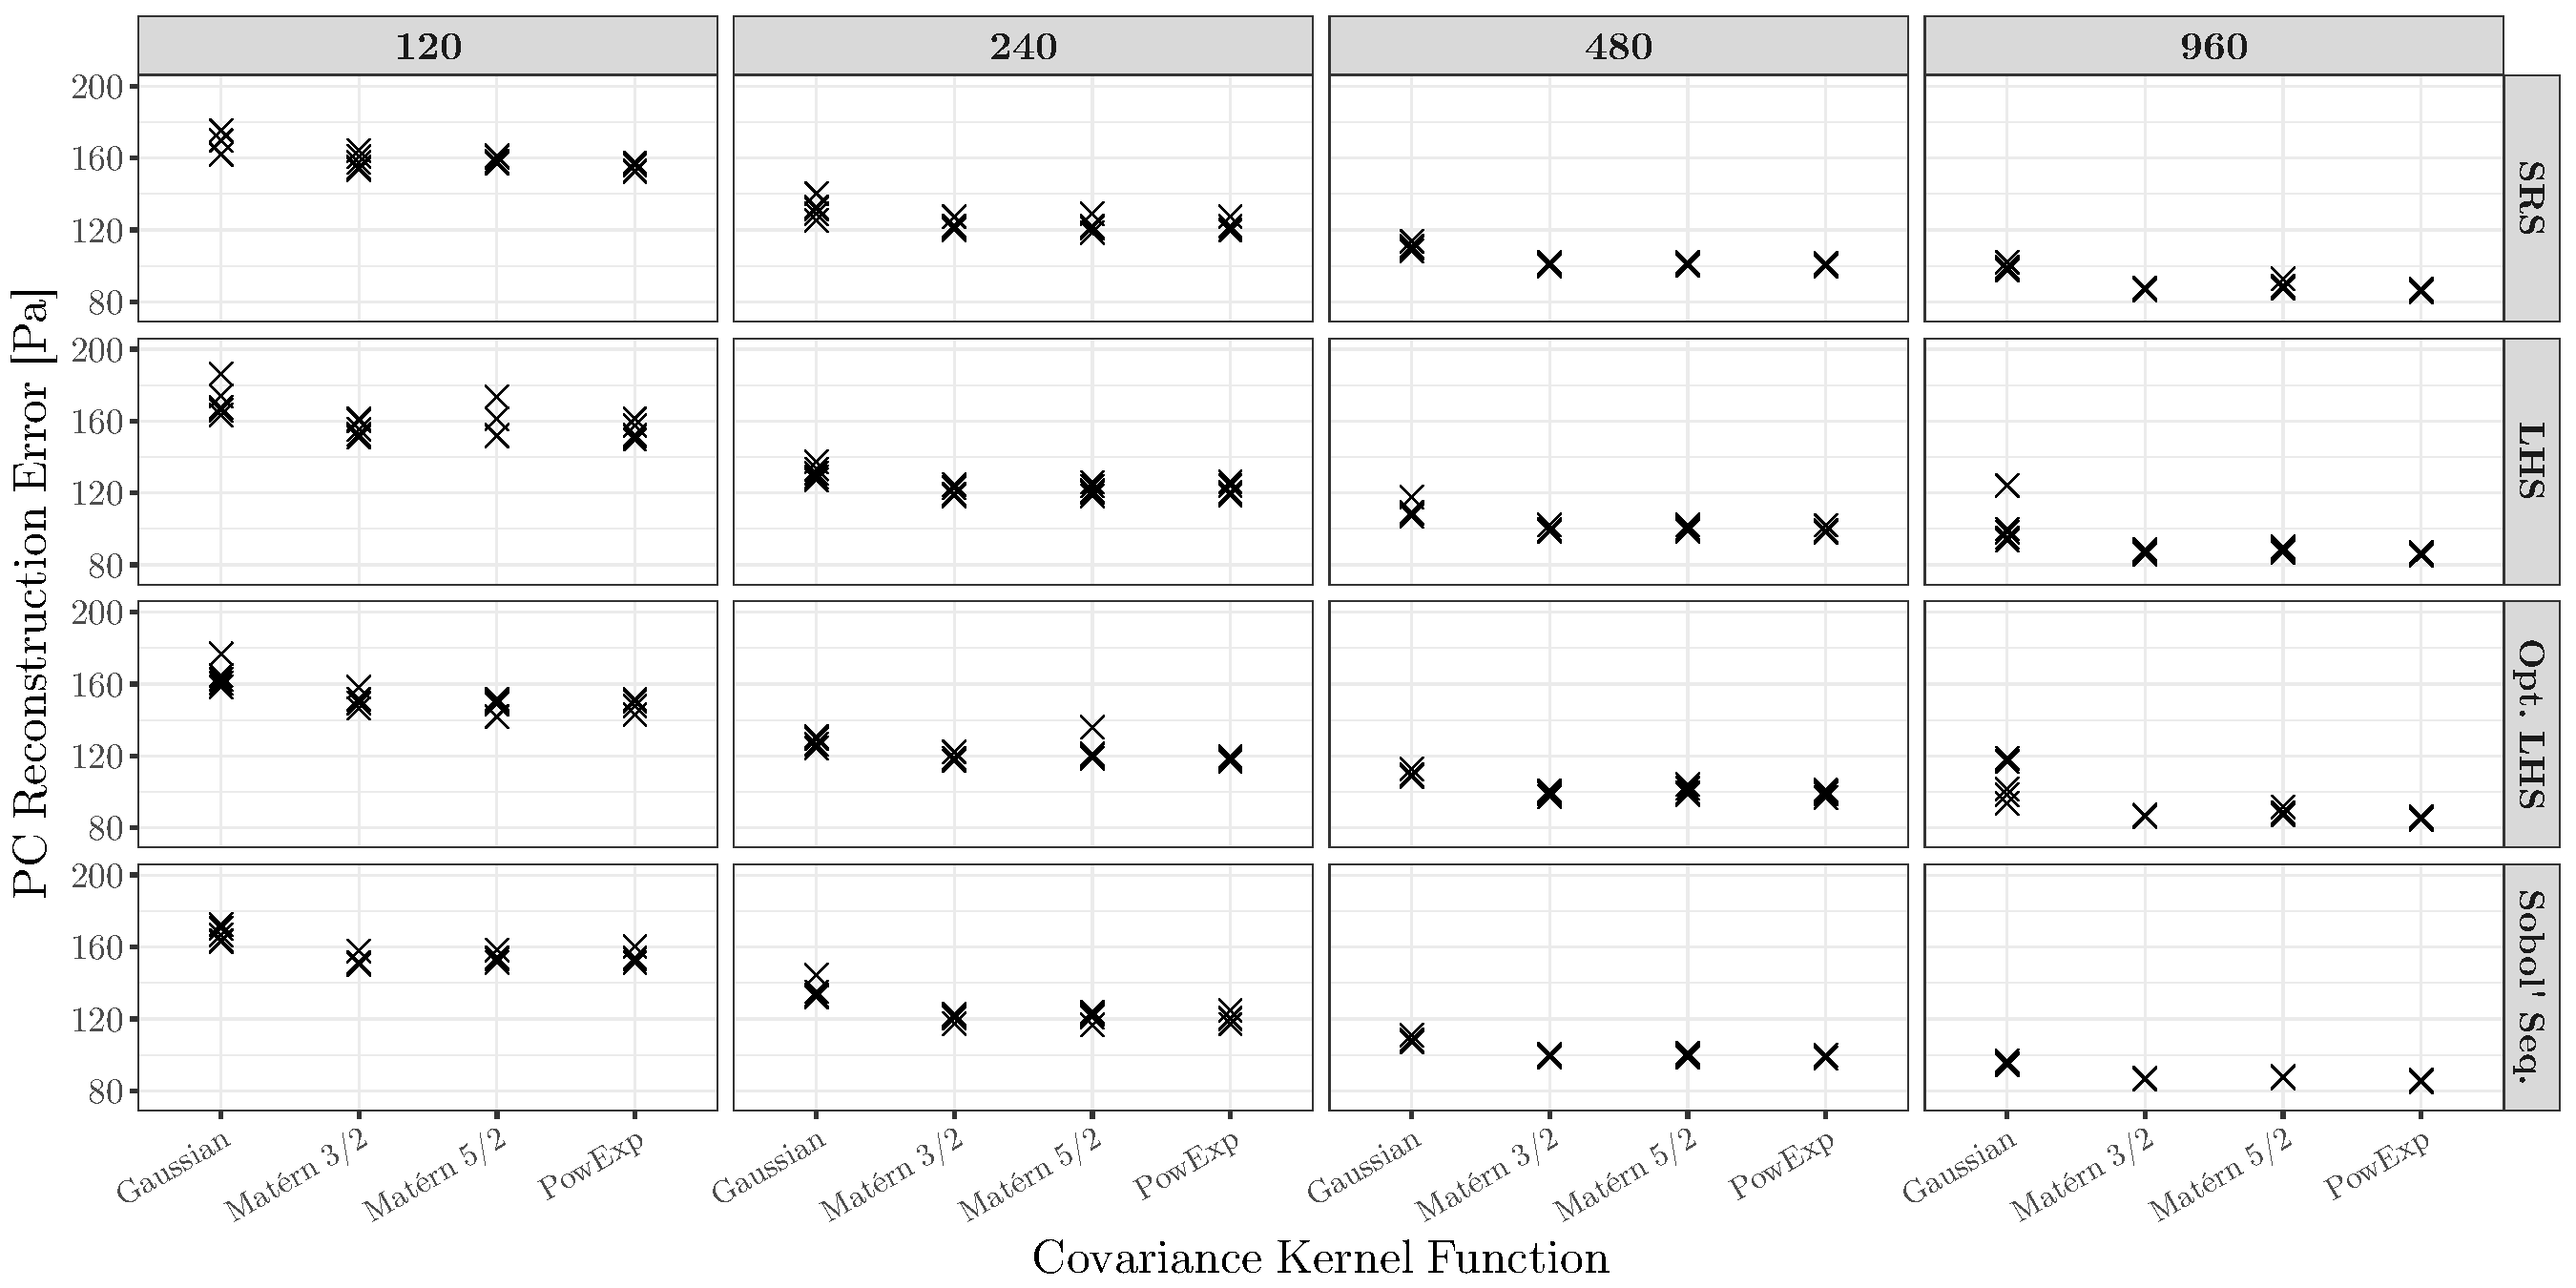
\includegraphics[width=1.0\textwidth]{../figures/chapter4/figures/plotPCGPConstructionDP}
	\caption[The flowchart for the implemented sensitivity analysis methodology applied to the TRACE model of FEBA facility]{The flowchart for the implemented sensitivity analysis methodology applied to the \gls{trace} model of \gls{feba} facility}
	\label{fig:ch4_plot_pc_gp_construction_dp}
\end{sidewaysfigure}

\bigfigure[pos=!tbhp,
					 opt={width=1.0\textwidth},
           label={fig:ch4_plot_pc_q2_dp},
           shortcaption={Sobol' Indices estimates with the scores of the warping function for the mid-height clad temperature transient as the \gls[hyper=false]{qoi}}]
{../figures/chapter4/figures/plotPCQ2DP}
{The sensitivity indices with respect to of the warping function for the mid-height clad temperature transient. Each boxplot represents the bootstrap sample quartile statistics and the vertical line extends the $95$th sample percentile.}

\begin{sidewaysfigure}
	\centering
	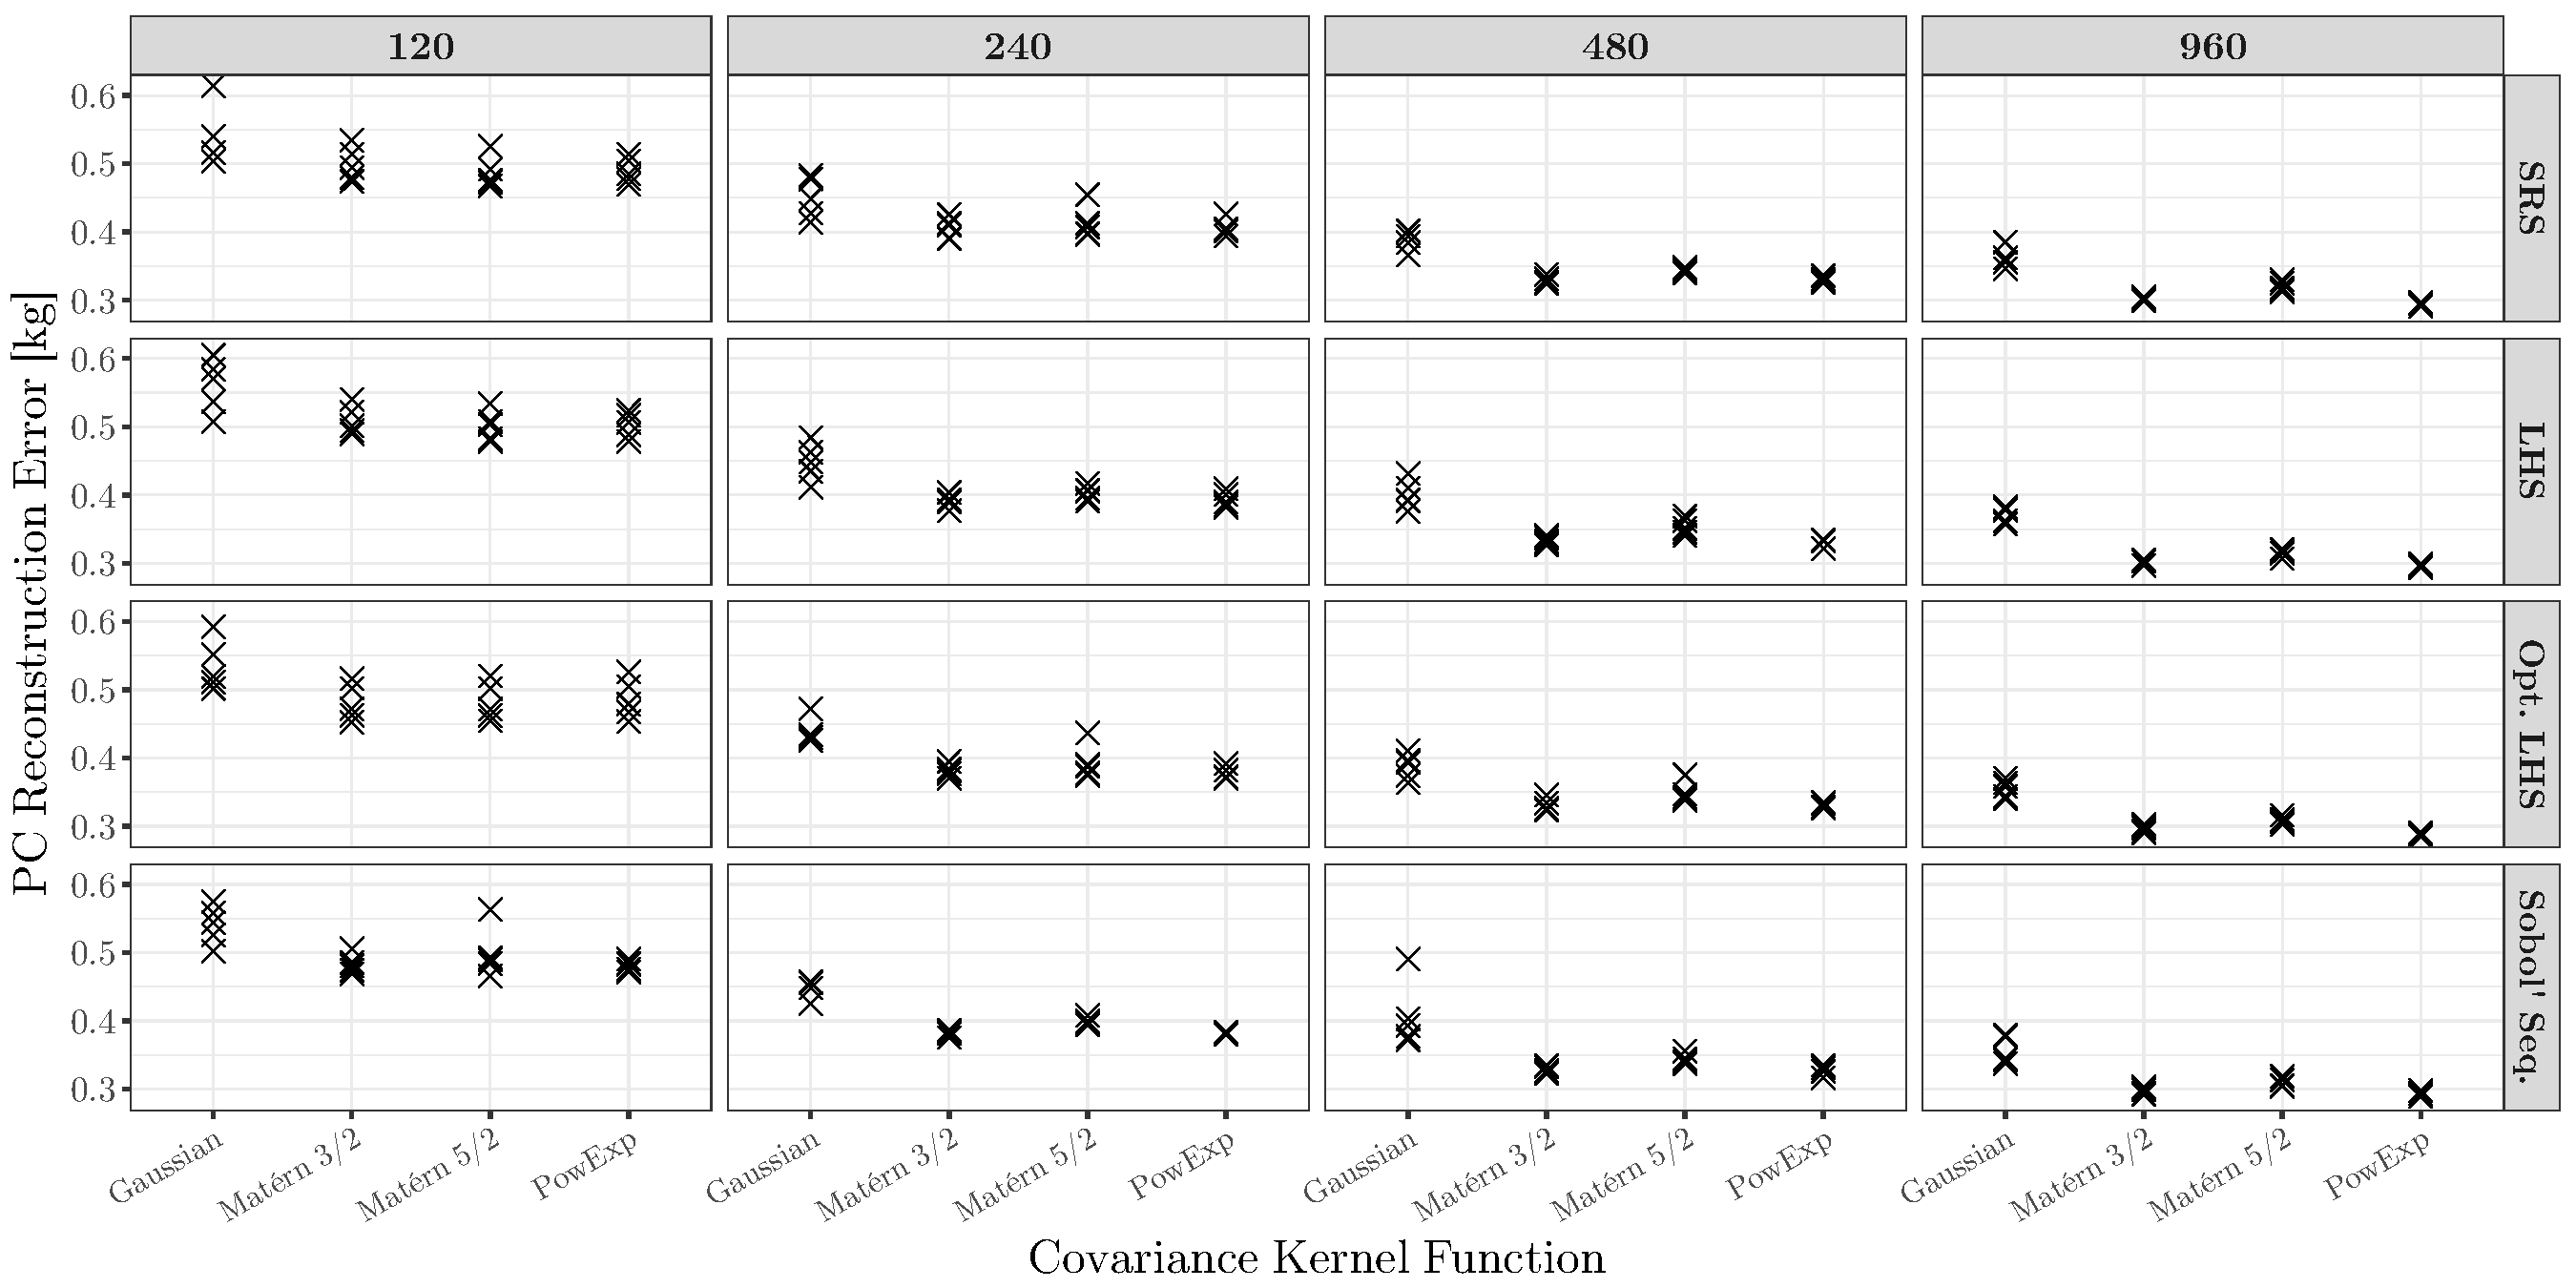
\includegraphics[width=1.0\textwidth]{../figures/chapter4/figures/plotPCGPConstructionCO}
	\caption[The flowchart for the implemented sensitivity analysis methodology applied to the TRACE model of FEBA facility]{The flowchart for the implemented sensitivity analysis methodology applied to the \gls{trace} model of \gls{feba} facility}
	\label{fig:ch4_plot_pc_gp_construction_co}
\end{sidewaysfigure}

\bigfigure[pos=!tbhp,
					 opt={width=1.0\textwidth},
           label={fig:ch4_plot_pc_q2_co},
           shortcaption={Sobol' Indices estimates with the scores of the warping function for the mid-height clad temperature transient as the \gls[hyper=false]{qoi}}]
{../figures/chapter4/figures/plotPCQ2CO}
{The sensitivity indices with respect to the of the warping function for the mid-height clad temperature transient. Each boxplot represents the bootstrap sample quartile statistics and the vertical line extends the $95$th sample percentile.}